%! Author = mariuszindel
%! Date = 02.11.20

\section{Delegates}

\subsection{Überblick}
\begin{itemize}
    \item Typsichere Funktions-Pointer
    \item Reference Type
    \item Intern Referenz auf 0-n Methoden
    \item Verwendung:
    \begin{itemize}
        \item Methoden als Parameter übergeben
        \item Definition von Callback-Methoden
    \end{itemize}
\end{itemize}

\subsubsection{Syntax}
\begin{itemize}
    \item Deklarieren eines Delegate Typs
    \begin{itemize}
        \item Schlüsselwort "delegate"
        \item Definition Rückgabewert
        \item Definition eines Namens
        \item Definition von Parameter
    \end{itemize}
\end{itemize}

\begin{lstlisting}
public delegate void Notifier(string sender);

class Examples {
    public static void Test() {

        // Deklaration Delegate-Variable
        Notifier greetings;

        // Zuweisung einer Methode
        greetings = new Notifier(SayHi);

        // Kurzform
        greetings = SayHi;

        // Aufruf einer Delegate-Variable
        greetings("John");
    }

    private static void SayHi(string sender) {
        Console.WriteLine("Hello {0}", sender);}}
\end{lstlisting}

\subsubsection{Verwendung / statisch}
\begin{center}
    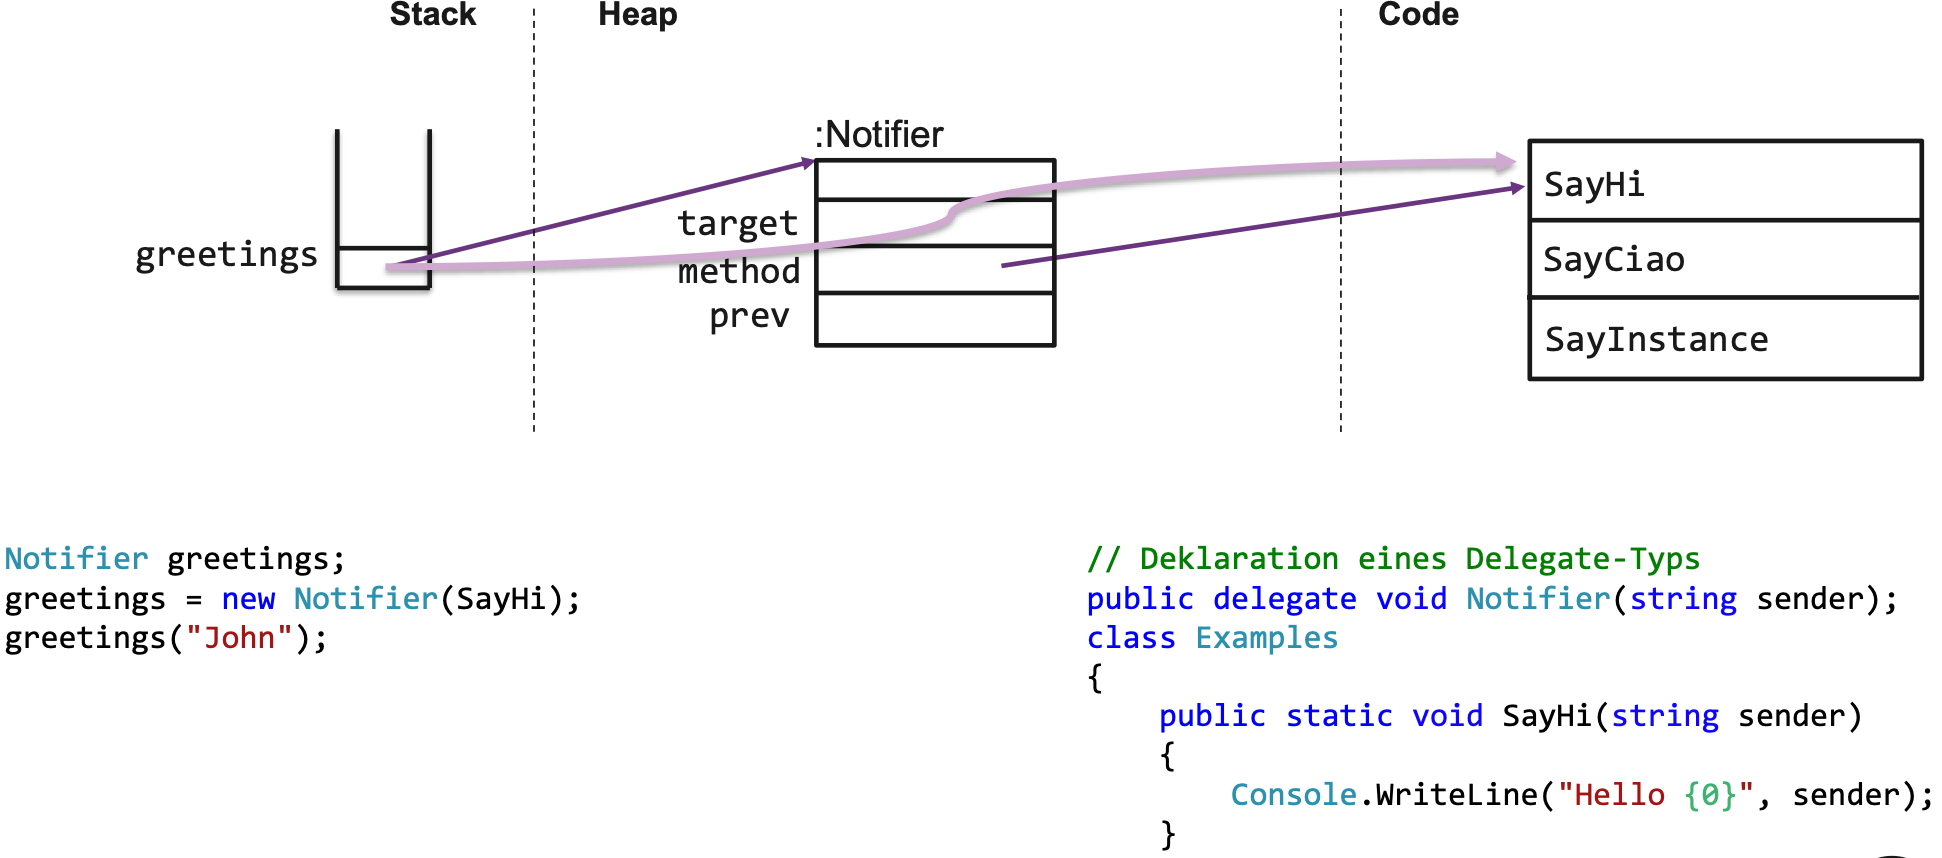
\includegraphics[scale=.26]{graphic/delegate/statisch.png}
\end{center}
\vspace{-8pt}

\subsubsection{Verwendung / Instanz}
\begin{center}
    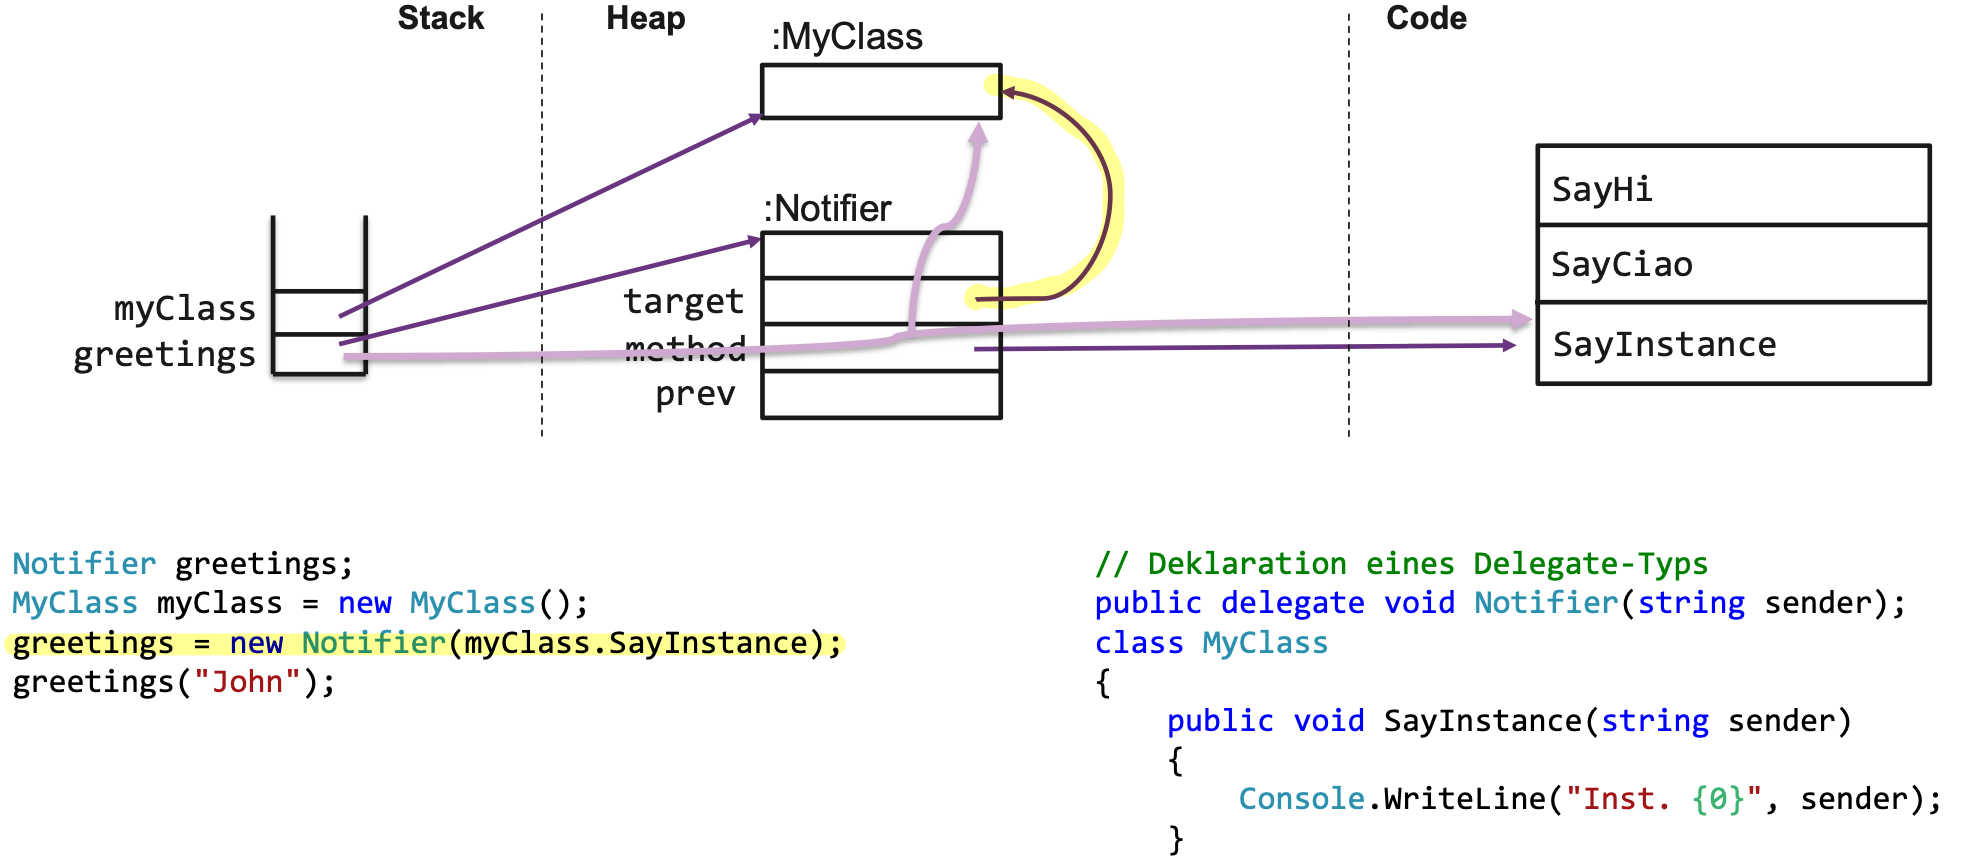
\includegraphics[scale=.26]{graphic/delegate/Instanz.png}
\end{center}
\vspace{-8pt}

\subsubsection{Zuweisung einer Methode}
Zuweisungs-Syntax:
\begin{lstlisting}
DelegateType delegateVar = obj.Method;
\end{lstlisting}

\begin{itemize}
    \item Ein Delegate speichert Methode (Method) und Empfänger-Objekt(obj)
    \item obj kann this bedeuten, deshalb weggelassen werden
    \item Method:
    \begin{itemize}
        \item kann static stein
        \item nicht abstract
        \item darf virtual, override und new sein
        \item muss mit Signatur von DelegateType übereinstimmen
    \end{itemize}
\end{itemize}

\subsubsection{Aufruf einer Delegate-Variable}
Aufruf-Syntax:
\begin{lstlisting}
object result = delegateVar[.Invoke](params);
\end{lstlisting}

\begin{itemize}
    \item Rückgabewert kann weiterverwendet werden falls nicht «void» (z.B. in Variable speichern)
    \item delegateVar darf nicht null sein / muss geprüft werden
    \begin{itemize}
        \item delegateVar?.Invoke(params);
    \end{itemize}
\end{itemize}

\subsection{Multicast Delegates}

\subsubsection{Übersicht}
\begin{itemize}
    \item  Jeder Delegate-Typ ist ein Multicast Delegate
    \item kann beliebig viele Methoden-Referenzen enthalten
    \item Zuweisung mit =
    \item Zuweisung mit +=
    \item Zuweisung mit -=
\end{itemize}
\begin{lstlisting}
public delegate void Notifier(string sender);

class Examples {

    public static void Test() {
        Notifier greetings;
        greetings = SayHi;
        greetings += SayCiao;
        greetings("John");
}

    private static void SayHi(string sender) {
    Console.WriteLine("Hello {0}", sender);}

    private static void SayCiao(string sender) {
    Console.WriteLine("Good bye {0}", sender);}
}
\end{lstlisting}

\subsubsection{Objektmodell}
Implementation in Form einer Linked List
\begin{itemize}
    \item target: Referenz auf Zielobjekt
    \item method: Methoden-Referenz
    \item prev: Referenz auf letztes Delegate
\end{itemize}

\vspace{-8pt}
\begin{center}
    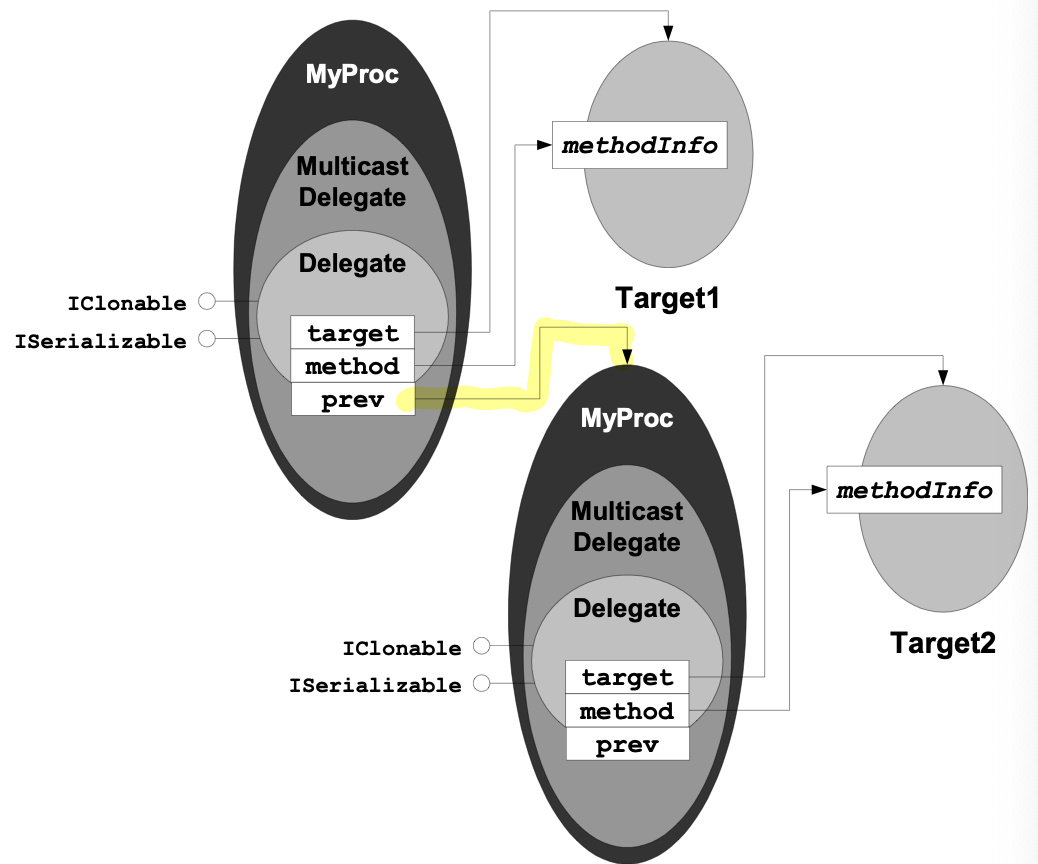
\includegraphics[scale=.34]{graphic/delegate/Objektmodell.png}
\end{center}
\vspace{-8pt}

\subsection{Funktionsparameter}
\begin{itemize}
    \item Methode für das Ausführen einer beliebigen Aktion auf jedem Element eines Arrays
    \item Ansatz: Funktion ForAll
    \begin{itemize}
        \item Int-Array mit Elementen
        \item Delegate mit auszuführender Funktion
    \end{itemize}
    \item Building Blocks
\end{itemize}

\begin{lstlisting}
public delegate void Action(int i);

public class MyClass {

    public static void PrintValues(int i)
    { Console.WriteLine("Value {0}", i); }

    public void SumValues(int i) { Sum += i; }
    public int Sum { get; private set; }
}

public class FunctionParameterTest {

    static void ForAll(int[] array, Action action)
    {
        Console.WriteLine("ForAll called...");
        if (action == null) { return; }
        foreach (int t in array) {
        action(t);
        }
    }
}
\end{lstlisting}

\subsection{Callback}

\subsubsection{Übersicht}

\begin{itemize}
    \item Tickende Uhr
    \begin{itemize}
        \item Benachrichtigung beim Ticken
        \item Subscribe / Unsubscribe Logik
    \end{itemize}
    \item Ansatz
    \begin{itemize}
        \item Clock-Objekt hält Liste von Callbacks
        \item Liste wird beim Ticken benachrichtigt
    \end{itemize}
    \item Implementation
    \begin{itemize}
        \item Interfaces
        \item Delegates
        \item Events
    \end{itemize}
\end{itemize}

\subsubsection{Implementation mit Delegates}
\begin{lstlisting}
public class ClockObserver {
    private string name;
    public ClockObserver(string name) { this.name = name; }

    public void OnTickEvent(int ticks, int i) {
    Console.WriteLine("Observer {0} : Clock mit Interval {2}
    hat zum {1}. Mal getickt.", name, ticks, i);}
}

public delegate void TickEventHandler (int ticks, int interval);
    public class Clock {
        private TickEventHandler OnTickEvent;
        public void add_OnTickEvent(TickEventHandler h) { OnTickEvent += h; }
        public void remove_OnTickEvent(TickEventHandler h) { OnTickEvent -= h; }
        private void Tick(object sender, EventArgs e) {
        ticks++; OnTickEvent?.Invoke(ticks, interval);}
}

public static void Test() {
    Clock c1 = new Clock(1000);
    Clock c2 = new Clock(2000);
    ClockObserver t1 = new ClockObserver("O1");
    ClockObserver t2 = new ClockObserver("O2");

    //Observers anmelden
    c1.add_OnTickEvent(t1.OnTickEvent);
    c2.add_OnTickEvent(t2.OnTickEvent);

    //Observers abmelden
    c1.remove_OnTickEvent(t1.OnTickEvent);
    c2.remove_OnTickEvent(t2.OnTickEvent); }
\end{lstlisting}